\documentclass[aspectratio=43]{beamer}

\usepackage{mathtools}

\usepackage{booktabs}
\usepackage{chemfig}
\usepackage{mhchem}

\usepackage{tikz}

\usepackage{xcolor}



\usepackage[sfdefault]{FiraSans} 

\definecolor{micmBand}{RGB}{188,226,230}
\definecolor{micmBlue}{RGB}{52,148,186} 
\definecolor{micmTeal}{RGB}{88,182,192}
\definecolor{micmGreen}{RGB}{117,189,167}
\definecolor{micmGray}{RGB}{122,140,142}
\definecolor{micmSlate}{RGB}{132,172,182}
\definecolor{micmDark}{RGB}{80,80,80}

\newcommand{\exersice}[1]{\colorbox{micmGreen!20}{{\color{red}\textbf{Hands On Task:}} \color{blue}\texttt{#1}}}

\mode<presentation>
{
  \usetheme{Madrid} 
  \setbeamertemplate{navigation symbols}{}
  \setbeamertemplate{caption}[numbered]  
  \setbeamercolor{structure}{fg=micmBand}
  \setbeamercolor{palette primary}{bg=micmBand, fg=white}
  \setbeamercolor{palette secondary}{bg=micmTeal, fg=white}
  \setbeamercolor{palette tertiary}{bg=micmGreen, fg=white}
}


% Define Title page

\setbeamertemplate{title page}{
    \begin{tikzpicture}[remember picture, overlay]
        \node[fill=micmBand,anchor=north, minimum height=0.20\paperheight, minimum width=\paperwidth] (headband) at (current page.north) {};
        \node[anchor=north east] (sponsor-cg) at (headband.south east)
        {\includegraphics[width=0.35\textwidth]{images/cccg-logo.png}};
        \node[anchor=north west] (sponsor-d2r) at (headband.south west) {\includegraphics[width=0.35\textwidth]{images/d2r-logo.png}};
        \node[anchor=west] (micm-logo) at (headband.west) {\includegraphics[width=0.45\textwidth]{images/micm-logo.png}};
        \node[anchor=east] (cdsi-logo) at (headband.east) {\includegraphics[width=0.35\textwidth]{images/cdsi-logo.png}};
        \node[] (title) at (current page.center) {\usebeamerfont{title}{\inserttitle}};
        \node[anchor=west] (name) at ([yshift=0.15\textheight]current page.south west) {\usebeamerfont{institute}{\textcolor{black}{\textbf{Workshop Lead: }\insertauthor}\par}};
        \node[anchor=north west] (date) at
        (name.south west)
         {\usebeamerfont{institute}{\textbf{Date: }\textcolor{black}{\insertdate}\par}};
    \end{tikzpicture}
 }


 % Define Template for each page

\newcommand{\micmlogofile}{images/micm-logo.png}
\setbeamertemplate{footline}{%
  \begin{beamercolorbox}[wd=\paperwidth, ht=0pt, dp=4mm, leftskip=1mm]{normal text}
\tiny\color{micmGray}\insertframenumber/\inserttotalframenumber
  \end{beamercolorbox}
  \begin{tikzpicture}[remember picture, overlay]
    \def\footlinewidth{0.32cm}
    \def\logoheight{0.8cm}
    \fill[micmBlue]  (current page.south west) rectangle ++(0.2\paperwidth,\footlinewidth);
    \fill[micmTeal]  ([xshift=0.2\paperwidth]current page.south west) rectangle ++(0.2\paperwidth,\footlinewidth);
    \fill[micmGreen] ([xshift=0.4\paperwidth]current page.south west) rectangle ++(0.2\paperwidth,\footlinewidth);
    \fill[micmGray]  ([xshift=0.6\paperwidth]current page.south west) rectangle ++(0.2\paperwidth,\footlinewidth);
    \fill[micmSlate] ([xshift=0.8\paperwidth]current page.south west) rectangle ++(0.2\paperwidth,\footlinewidth) coordinate (corner);
    \node[anchor=south east, inner sep=0pt] at (corner)
      {\includegraphics[height=\logoheight]{\micmlogofile}};
    \node[red,draw] at ([xshift=0.5cm]corner) {\insertframenumber/\inserttotalframenumber};
  \end{tikzpicture}%
}

\AtBeginSection[]{
  \begin{frame}
    \centering
    \usebeamerfont{title}\insertsectionhead
  \end{frame}
}

\author[Tabish]{Tabish Syed}
\institute[McGill]{McGill University}
\title[Latex Workshop]{Writing With \LaTeX{}}
\date{October 30th, 2026}

\begin{document}
\maketitle

\section{Introduction}
\begin{frame}{Introduction}

            \begin{itemize}
                \item<1-> \LaTeX{} is a \emph{markup language} for typesetting documents.
                \item<2-> Unlike WYSIWYG (what you see is what you get) word processors, in \LaTeX{} you write the \emph{content and structure} in plain text.
            \end{itemize}
        \uncover<3->{
        \begin{center}  
        \begin{tabular}{lll}
        \toprule
        You write (source \texttt{.tex}) & & You get (compiled \texttt{.pdf})\\
        \midrule
        \texttt{E = mc\textasciicircum 2} & $\Rightarrow$ & $E = mc^2$ \\
        \texttt{\textbackslash section\{Intro\}} & $\Rightarrow$ & ``1\quad Introduction'' \\
        \texttt{\textbackslash alpha, \textbackslash infty} & $\Rightarrow$ & $\alpha, \infty$ \\
        \bottomrule
        \end{tabular}
        \end{center}
        }     
\end{frame}

\begin{frame}{Getting set up}
\begin{itemize}
  \item<1-> \textbf{Easiest:} \href{https://www.overleaf.com}{Overleaf} --- online,
        no installation, shared editing, built-in compiler.
  \item<2-> \textbf{Local install:} TeX Live (\textsc{mac}/Linux) or MiKTeX (Windows).
        Compile from a terminal with \texttt{pdflatex file.tex} or
        \texttt{latexmk -pdf file.tex}.
  \item<3-> \textbf{Editors:} any text editor; popular ones add syntax highlighting and one-click compile (TeXMaker, VS Code + LaTeX Workshop).
\end{itemize}
\end{frame}

\begin{frame}{First \LaTeX{} Document}
  \textbackslash \texttt{documentclass[options]}\{ \}\\
  \textbackslash \texttt{begin\{document\}}\\
  \hspace{2mm}$\cdots$\\
  \textbackslash \texttt{end\{document\}}

  \vspace{5mm}

  \uncover<2->{
    \begin{center}
    \begin{tabular}{@{}ll@{}}
    \toprule
    Class & Typical use\\
    \midrule
    \texttt{article} & journal papers, reports, homework\\
    \texttt{report} & longer documents, chapters allowed\\
    \texttt{book} & books, thesis\\
    \texttt{beamer} & presentation slides\\
    \bottomrule
    \end{tabular}
    \end{center}
    Class options in square brackets: \texttt{11pt}, \texttt{a4paper},
    \texttt{twocolumn}, \texttt{draft}. 
  }

  \uncover<3->{
    \begin{center}
        \exersice{Create New Project On Overleaf}
    \end{center}
  }
\end{frame}

\begin{frame}{Compilation}
    \begin{itemize}
  \item \texttt{pdflatex paper.tex} $\to$ \texttt{paper.pdf} (first pass; collects
        references into \texttt{.aux})
  \item \texttt{bibtex paper} $\to$ reads \texttt{.aux} + \texttt{refs.bib},
        writes \texttt{.bbl}
  \item \texttt{pdflatex} twice more $\to$ resolves citations and cross-references
\end{itemize}

\vspace{1cm}

\uncover<2->{
Alternatively, press the \texttt{Ctrl+Enter} or click `\texttt{Recompile}' in \texttt{overleaf}
}

\uncover<2->{
\begin{center}
    \exersice{Try on overleaf}
\end{center}
}

\end{frame}

\begin{frame}{Document Structure}
\begin{center}
\uncover<1->{\exersice{Exercises/001-SimpleText.tex}}

\vspace{1cm}

\uncover<2->{\exersice{Exercises/002-StructuredDocument.tex}}

\vspace{1cm}

\uncover<3->{\exersice{Exercises/004-AddingReferences.tex}}
\end{center}

\end{frame}

\section{Images}

\begin{frame}{Single Image Figures}
    \begin{center}
        \exersice{Exercises/100-SingleImages.tex}
    \end{center}
\end{frame}

\begin{frame}{Multi-Panel Images}
    \begin{center}
        \exersice{Exercises/101-ImageGrid.tex}
    \end{center}
\end{frame}


\section{Drawings}
\begin{frame}{Drawings}
    \begin{center}
    \only<1-2>{
        \exersice{Exercises/102-TikzDrawings.tex}

        \vspace{1cm}
        
        \uncover<2>{
        \exersice{Exercises/103-StandaloneAnnotatedFigure.tex}
        }
    }
    \includegraphics<3>[width=\textwidth]{images/synapse.pdf}
    \end{center}
\end{frame}

\section{Appendix}

\begin{frame}{Anotated Equations}
    \begin{equation}
  %\tikzexternaldisable
  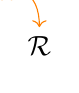
\begin{tikzpicture}[baseline=(t.base)]
    \path[use as bounding box] node[inner xsep=0em] (t) {$\mathcal{R}$};
    \draw[orange,<-] (t.north) to[out=90,in=0] ++(120:0.5)
    node[left,inner sep=0.1em,font=\footnotesize]{Rate};
  \end{tikzpicture}
  %
  \approx
    \overbrace{\sum_{\ell=1}^r}^{{\color{green!50!black}Collect}} \,
  %
  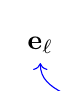
\begin{tikzpicture}[baseline=(a.base)]
      \path[use as bounding box] node[inner xsep=0em] (a) {$\mathbf{e}_{\ell}$};
      \draw[blue,<-] (a.south) to[out=-90, in=120] ++(-45:1.0) node [below, inner sep=0.1em, font=\footnotesize]{Enzyme};
  \end{tikzpicture}
  \circ
  %
  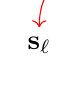
\begin{tikzpicture}[baseline=(c.base)]
    \path[use as bounding box] node[inner xsep=0em] (c) {$\mathbf{s}_{\ell}$};
    \draw[red,<-] (c.north) to[out=90,in=180] ++(60:0.6)
    node[right,inner sep=0.1em,font=\footnotesize]{Substrate};
  \end{tikzpicture}
\end{equation}
\end{frame}


\begin{frame}{Chemical Drawings}
    Behold, the grand caravan of amino acids marched briskly through the meadows of Alanin, each one wearing a tiny hat made of peptides and whispering secrets to the wind.
    \chemfig[chemfig style={scale=0.5}, atom style={scale=0.5}, scheme gap=5em]{H_2N-C(<[2]CH_3)(<:[6]H)-C(=[1]O)-[7]OH} Leucine, feeling particularly spherical, declared itself Emperor of the Pancake and demanded that all side chains be flushed weekly with \ce{H2O}. Meanwhile, benzene \chemfig[chemfig style={scale=0.2}, atom style={scale=0.2}]{**6(------)} - the shy, smallest cousin rolled seven invisible phenols  \chemfig[atom sep=1.2em, atom style={scale=0.5}]{*6(-(-OH)=-=-=)} while humming a tune in the key of Tyrosine codon \ce{H2N-CH3-CO-CH3} table was just a very reactive crossword puzzle invented by bored mitochondria \chemfig[chemfig style={scale=0.3}, atom style={scale=0.3},scheme gap=2em]{H_2N-CH(-[6]C(=[5]O)-[7]OH)-CH_2-**6(---(-OH)---)}
\end{frame}

\begin{frame}
    \begin{center}
        \begin{tabular}{cc}
        
\includegraphics[width=0.2\textwidth]{images/workshop-feedback-qr.png} &
        \includegraphics[width=0.2\textwidth]{images/micm-mailing-list-qr.png}\\
        Workshop Feedback & MiCM Mailing List
        \end{tabular}
    \end{center}
\end{frame}

\end{document}